\section{Strong NP-completeness}
\label{sec:hardness}

The approximation algorithms exploit planar structure, but exact
optimization remains hard. We first state the decision and source
problems and the graph terminology used by both reductions.

\begin{definition}[Complexity and reductions]\label{def:complexity}
A \emph{polynomial-time many-one reduction} maps instances of one
decision problem to another in polynomial time, so an input is a
yes-instance if and only if its image is a yes-instance.

A decision problem is in \emph{NP} if every yes-instance has a
certificate of polynomial encoding length whose validity is
checkable in polynomial time, and no certificate is accepted on a
no-instance. It is \emph{NP-hard} if every problem
in NP admits such a reduction to it, and \emph{NP-complete} if it
is both NP-hard and in NP.
A numerical problem is \emph{strongly NP-hard} if hardness persists
when its integer data are bounded by a fixed polynomial in the
combinatorial instance size; it is \emph{strongly NP-complete} if
it is also in NP. For rational data, our restricted instances
explicitly bound both numerators and denominators.
\end{definition}

\begin{definition}[3-Partition]\label{def:three-partition}
The input consists of positive integers $a_1,\ldots,a_m,B$, where
$m=3p$ for a positive integer $p$, satisfying
\[
 s=\sum_{i=1}^m a_i=pB,\qquad B/4<a_i<B/2.
\]
The question is whether $[m]$ can be partitioned into $p$ groups
$I_1,\ldots,I_p$ with $|I_b|=3$ and
$\sum_{i\in I_b}a_i=B$ for every $b$.
\end{definition}

\begin{symboltable}
$m=3p,\ [m]$ & Number of source items and their index set.\\
$a_i,\ B$ & Item size $i$ and target sum of each bin.\\
$s=pB=\sum_i a_i$ & Total item size and total capacity of the $p$ bins.\\
$I_b$ & Index set of the three items assigned to source bin $b$.\\
\end{symboltable}

Both reductions use the strong NP-completeness of this
problem~\cite{gj1979}.
We use the NP-hard restriction in which $B$ is polynomially bounded
in $m$. The case $p=1$ is a trivial yes-instance, so excluding it
preserves NP-hardness. In this restriction each $a_i$ is
polynomially bounded, so the explicit
repetitions in our constructions remain polynomial in the source
size. A partition into $p$ groups of sum $B$
then necessarily has three items per group: two items sum to less
than $B$, while four items sum to more than $B$.

\begin{definition}[Paths and matchings]\label{def:paths-and-matchings}
A \emph{path} is an undirected graph with distinct vertices
$v_0,\ldots,v_k$ and edges exactly
$\{v_{j-1},v_j\}$ for $1\le j\le k$.
A \emph{linear forest} is a disjoint union of paths, allowing
isolated vertices. In this paper an \emph{odd path} has an odd
number of vertices, not an odd number of edges.
Odd and even positions refer to local positions numbered from zero
along an item path, not to global hypothesis indices.

A \emph{matching} is a set of edges with no shared endpoint.
A vertex is \emph{unmatched} if it is incident to no chosen edge.
A \emph{maximum matching} has largest possible cardinality;
``maximum'' here always refers to the number of edges, not their
weights. A \emph{perfect matching} leaves no vertex unmatched.
\end{definition}

The two reductions share a combinatorial mechanism. They place each
item on an odd path and supply singleton and adjacent-pair membership
tests. A maximum matching leaves one even-position vertex unmatched;
its position chooses the item's bin. Moving that position changes
a short part of a histogram. The maximum-depth reduction counts
branch heights, while the expected-depth reduction counts pair weights.
In both cases these local changes add to the source bin loads.

\subsection{The geometric realization and the matching choice}

For integer abscissae, the line
\[
 I_{a,b}:\quad
 4y-4(a+b)x+(2a-1)(2b+1)=0
\]
has value $4(x-a+\tfrac12)(x-b-\tfrac12)$ on $(x,x^2)$.
Its negative answer selects exactly the integer abscissae
$a,\ldots,b$. This realizes interval membership using one line.
The line
\begin{equation}\label{eq:private-singleton}
 P_t:\quad 2y-4tx+2t^2-1=0
\end{equation}
has value $2(x-t)^2-1$, and its negative answer isolates exactly
the point of abscissa $t$. Both formulas are nonzero at all integer
abscissae, so every answer is binary.
The tangent $y=2tx-t^2$ exposes the point $(t,t^2)$, since every
other parabola point lies strictly above it. The constructed
hypotheses are therefore in strictly convex position.

In both reductions, membership sets are the negative answer classes
of the displayed lines. Thus a hit in
Definition~\ref{def:membership-spine} is the negative affine sign;
the distinguished hypothesis misses these sets. The query itself
is unchanged.



These formulas provide the two query types needed by the reduction:
an interval query selects a consecutive block, and a private
singleton query distinguishes one point from all the others.
Putting the points on a parabola gives both query types with integer
coefficients while keeping every hypothesis exposed on the convex
hull. For example, Figure~\ref{fig:parabola-queries} shows
$I_{2,5}$ and $P_4$ on the points with integer abscissae from $0$ to $8$.

\begin{figure}[tbp]
\centering
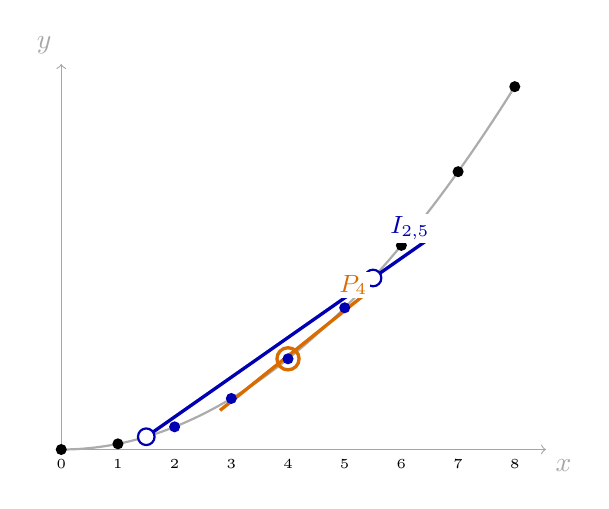
\begin{tikzpicture}[x=0.72cm,y=0.072cm]
  \draw[->,gray!70] (0,0)--(8.55,0) node[below right] {$x$};
  \draw[->,gray!70] (0,0)--(0,68) node[above left] {$y$};
  \foreach \x in {0,...,8} {
    \node[below,font=\tiny] at (\x,0) {\x};
  }
  \draw[thick,gray!65] plot[domain=0:8,samples=81] (\x,{(\x)^2});
  \draw[very thick,blue!70!black]
    plot[domain=1.5:6.5,samples=60] (\x,{7*\x-8.25});
  \draw[very thick,orange!85!black]
    plot[domain=2.8:5.4,samples=50] (\x,{8*\x-15.5});
  \draw[blue!70!black,fill=white,thick] (1.5,2.25) circle (3pt);
  \draw[blue!70!black,fill=white,thick] (5.5,30.25) circle (3pt);
  \foreach \x in {0,1,6,7,8} {
    \pgfmathsetmacro{\yy}{\x*\x}
    \fill[black] (\x,\yy) circle (2pt);
  }
  \foreach \x in {2,3,4,5} {
    \pgfmathsetmacro{\yy}{\x*\x}
    \fill[blue!70!black] (\x,\yy) circle (2pt);
  }
  \draw[orange!85!black,very thick] (4,16) circle (4pt);
  \node[font=\small,text=blue!70!black,fill=white,inner sep=1pt]
    at (6.15,39) {$I_{2,5}$};
  \node[font=\small,text=orange!85!black,fill=white,inner sep=1pt]
    at (5.15,29) {$P_4$};
\end{tikzpicture}
\caption{The integer points lie on $y=x^2$. The blue line
$I_{2,5}$ has negative answer exactly on the points with
$x\in\{2,3,4,5\}$; the orange line $P_4$ has negative answer only
at $x=4$, marked with an orange ring. The interval endpoints are
the half-integer intersections $x=1.5$ and $x=5.5$.}
\label{fig:parabola-queries}
\end{figure}

For maximum depth we also use \emph{clouds} of ordinary points.
They make a local identification problem take a chosen number of
queries without changing the objective. A cloud's size $w_i$ is
its number of points, not a prior weight.
Given positive integer cloud sizes $w_i$, put $Q=4\max_i w_i$
and represent cloud $i$ by
\[
 \{(Qi+j,(Qi+j)^2):0\le j<w_i\}.
\]
Its point with $j=0$ is its \emph{anchor}. Supply the cloud-interval line
\begin{equation}\label{eq:cloud-interval}
 4y-4Q(a+b)x+Q^2(2a-1)(2b+1)=0.
\end{equation}
For $a\ge1$ its negative answer selects exactly the clouds
$a,\ldots,b$, while excluding cloud $0$.
This follows by factoring its value as
$4(x-Q(a-\tfrac12))(x-Q(b+\tfrac12))$.
Each cloud lies within $Q/4$ of its anchor, so neither boundary,
halfway between consecutive anchors, contains a hypothesis.
We supply private lines \eqref{eq:private-singleton} for each
nonanchor point, but not for the anchors. An anchor and a point
in its own cloud agree on every cloud-interval test and on every
other private test. Their separation requires that point's
private query. Thus a cloud of size $w$ forces $w-1$ queries on
the anchor's local path, while the anchor itself remains available
to represent the cloud in the matching construction.

Clouds are ordered so that consecutive vertices of each path used
below have consecutive cloud indices. The only cloud-interval tests
are whole-cloud singleton tests and adjacent-pair tests specified
by those paths. Every point, including every anchor, must be identified.

\begin{lemma}[Identifying one or two clouds]\label{lem:cloud-heights}
For this supplied family, the minimum height on one cloud of size $w$
is $w-1$. On two clouds of sizes $u,v$, when their whole-cloud
singleton tests are supplied, the minimum height is $\max\{u,v\}$.
\end{lemma}
\begin{proof}
On a single cloud, old cloud-interval tests are constant and each
private test isolates one nonanchor point. The anchor answers the
same way as every nonanchor on all the other private tests, so its
path must ask all $w-1$ of them. Querying them sequentially achieves
that height.

On two clouds, the anchor of the larger cloud must use all its
private tests: each is the only query separating that cloud's anchor
from its corresponding nonanchor. It must also use at least one
cloud-interval test, since private tests give the same answer at
both anchors. The larger cloud therefore forces depth at least
$\max\{u,v\}$.
First separating the clouds and then performing their private
searches attains the bound.
\end{proof}

\begin{lemma}[One unmatched position]\label{lem:odd-path}
A maximum matching of the path
\[
 E_0,B_1,E_1,\ldots,B_t,E_t
\]
leaves exactly one vertex $E_k$ unmatched. It then uses pairs
$\{E_{j-1},B_j\}$ for $j\le k$ and
$\{B_j,E_j\}$ for $j>k$.
\end{lemma}
\begin{proof}
The maximum size is $t$, so exactly one vertex is unmatched.
Both sides of that vertex must have even length, forcing it
to be an $E_k$. Each remaining even path has a unique perfect
matching: its endpoint must match its only neighbor, and induction
fixes the rest. This gives the displayed pairs.
\end{proof}

Figure~\ref{fig:odd-path-matching} shows the smallest nontrivial
example of the matching pattern. Moving the unmatched even-position
cloud changes which segment represents the item's bin choice.
\begin{figure}[tbp]
\centering
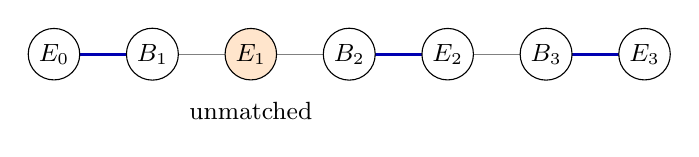
\begin{tikzpicture}[every node/.style={font=\small}]
  \draw[gray] (0,0)--(7.5,0);
  \draw[very thick,blue!70!black] (0,0)--(1.25,0);
  \draw[very thick,blue!70!black] (3.75,0)--(5,0);
  \draw[very thick,blue!70!black] (6.25,0)--(7.5,0);
  \node[draw,circle,fill=white,inner sep=2pt] at (0,0) {$E_0$};
  \node[draw,circle,fill=white,inner sep=2pt] at (1.25,0) {$B_1$};
  \node[draw,circle,fill=orange!20,inner sep=2pt] at (2.5,0) {$E_1$};
  \node[draw,circle,fill=white,inner sep=2pt] at (3.75,0) {$B_2$};
  \node[draw,circle,fill=white,inner sep=2pt] at (5,0) {$E_2$};
  \node[draw,circle,fill=white,inner sep=2pt] at (6.25,0) {$B_3$};
  \node[draw,circle,fill=white,inner sep=2pt] at (7.5,0) {$E_3$};
  \node[below=14pt] at (2.5,0) {unmatched};
\end{tikzpicture}
\caption{A maximum matching of
$E_0,B_1,E_1,B_2,E_2,B_3,E_3$ with $E_1$ left unmatched.
Blue edges are the selected adjacent pairs. In the reduction, the
unmatched even-position cloud selects the item's bin; the uniquely
forced pairs lie to its left and right.}
\label{fig:odd-path-matching}
\end{figure}

The item paths only organize the supplied membership queries. The
reduction uses singleton and adjacent-pair tests directly; no
underlying edge-query search tree is part of the instance.

\subsection{Maximum depth: bin loads become branch-height counts}

The construction has three jobs. A distinguished anchor forces the
spine to use a maximum matching. Only a few small even-position
clouds can be left unmatched, giving exactly $p$ bin choices per
item. Finally, the heights of the matched pairs record how much
load was assigned to each bin.

\begin{theorem}[Strong NP-completeness of maximum depth]
\label{thm:strong-worst}
Deciding whether $\OPT_{\mathrm W}(\HH)\le K$ is strongly NP-complete,
even for integer-coordinate points on a parabola, polynomially
bounded integer line coefficients, and $O(n)$ supplied binary
line queries.
\end{theorem}
\begin{proof}
For the source instance define
\[
 \begin{split}
 q&=(p-1)(4s+2m),\qquad M=m+2,\qquad K=q+M,\\
 T&=s-B,\qquad
 \lambda_1=M,\qquad
 \lambda_b=M+(2b-3)s\quad(2\le b\le p),\\
 H&=M+2s(p-1),\qquad C=H+1.
 \end{split}
\]
Here $q$ will be the total number of matched pairs and $K$ the
minimum length of the distinguished anchor's path.
The numbers $\lambda_b$ mark histogram levels for bins, and
$T$ is the width of each bin's window. The larger sizes $H,C$
keep the remaining pairs above those windows.

\begin{symboltable}
$q,\ K$ & Total number of matched pairs in a maximum matching and target maximum depth.\\
$M=m+2$ & Auxiliary-cloud size and offset used for the minimum bin level.\\
$T=s-B,\ \lambda_b$ & Width of each bin's histogram window and its lower level.\\
$H,\ C=H+1$ & Higher pair and connector exit heights, above every bin window.\\
$s_i=(p-1)(4a_i+2)$ & Number of odd-position clouds, and maximum matching size, in item $i$'s path.\\
\end{symboltable}

For item $i$, construct an odd path whose vertices represent clouds.
Starting with an even-position cloud of size $2$, append $p-1$
segments, indexed by $b=1,\ldots,p-1$. Each row below appends an
odd-position cloud and then the next even-position cloud.
Segment $b$ consists of one entry row, $a_i$ repetitions of the
four block rows, and one exit row:
\[
 \begin{array}{c|c|c}
 \text{part}&\text{odd-position size}&\text{next even size}\\ \hline
 \text{entry}&C&M\\
 \text{block step 1}&\lambda_b&H\\
 \text{block step 2}&\lambda_b+T&M\\
 \text{block step 3}&\lambda_{b+1}+T&H\\
 \text{block step 4}&\lambda_{b+1}&M\\
 \text{exit}&C&2
 \end{array}
\]
The repeated block is the only part depending on $a_i$.
It transfers $a_i$ units between neighboring histogram windows.
There are $4a_i+2$ odd-position vertices per segment, so the
whole item path has $2s_i+1$ vertices, where
$s_i=(p-1)(4a_i+2)$, and its maximum matching has size $s_i$.
Its $p$ even-position clouds of size $2$ are the segment boundaries.

Add one auxiliary cloud of size $M$ and cloud $0$ of size $2$.
Supply each nonzero cloud's whole-cloud singleton test, each
adjacent-pair test within an item path, and each nonanchor point's
private singleton test. Realize them by \eqref{eq:cloud-interval}
and \eqref{eq:private-singleton}.

\paragraph{Step 1: a tight distinguished path forces a matching.}
\begin{claim}[The distinguished path forces maximum matchings]
Every identifying tree has height at least $K$. If its height is at
most $K$, the first-covered pairs form a maximum matching in every
item path, and no nonzero-cloud private test is asked on the anchor
path.
\end{claim}
\begin{proof}
Follow the anchor of cloud $0$ through any complete tree. It needs the private
test for the other point of cloud $0$. Private tests of other
clouds do not distinguish their anchors from this anchor.
It therefore also needs cloud queries covering the $2q+m$ item-path
anchors and the auxiliary anchor.

Classify each anchor by its first hitting cloud query along this
all-miss path. A query first covers one anchor or two adjacent
anchors. The first-covered pairs are disjoint, hence form a
matching of size at most $\sum_i s_i=q$.
There are $2q+m+1$ nonzero anchors to cover. If $g$ first-covered
groups are pairs, the remaining groups are singletons, so the path
uses $(2q+m+1)-g$ cloud queries. Since $g\le q$, this is at least
$q+m+1$. It must also ask the private query separating the two
points of cloud $0$, giving the lower bound
$q+m+2=K$.

If a tree has height at most $K$, equality holds. No private test
of a nonzero cloud can occur on this path, and its pairs form a
maximum matching in every item path. Lemma~\ref{lem:odd-path}
therefore leaves exactly one even-position cloud unmatched per item.
\end{proof}

At this equality, all clouds are intact when first encountered:
none of their private points was removed earlier. A hit exit
contains one full cloud or two full clouds.
Replace any query first covering just one cloud by its supplied
whole-cloud singleton test. Put cloud $0$'s private query last;
this advances the other exits and leaves its two points within
depth $K$. Attach the optimal local codes of
Lemma~\ref{lem:cloud-heights}.

\paragraph{Step 2: summarize the remaining tree by a histogram.}
\begin{claim}[The sorted exit profile characterizes depth]
After the cloud-query groups are sorted by nonincreasing local
height, every target path has depth at most $K$ exactly when
$t+N(t)\le K$ at every exit-height level $t$.
\end{claim}
\begin{proof}
The cloud queries now act on disjoint singletons and pairs.
Their exit heights are $w-1$ for a singleton and $\max\{u,v\}$
for a pair. Include the final private query as an exit of height
zero. Sorting these heights in nonincreasing order cannot hurt:
exchanging consecutive heights $r<s$ replaces
$\max\{j+r,j+1+s\}$ by $\max\{j+s,j+1+r\}$.

Write $h_j$ for the local height of the exit at spine position $j$.
The \emph{tail histogram} of exit heights is
$N(t)=|\{j:h_j\ge t\}|$, the number of exits of height at least $t$.
In sorted order, the last such exit occurs at position $N(t)$.
An exit at position $j$ with local height $h_j$ has total depth
$j+h_j$. Because the heights are sorted, the maximum of these sums
is exactly the maximum of $t+N(t)$ over exit-height levels $t$:
an exit of height $t$ occurs no later
than position $N(t)$, and the last exit counted by $N(t)$ has height
at least $t$. Thus all target paths fit within $K$ exactly when
\begin{equation}\label{eq:height-profile}
 t+N(t)\le K
\end{equation}
for every exit-height level $t$.
This criterion is simply the maximum of ``spine position plus
remaining local depth.''
\end{proof}

\paragraph{Step 3: only boundaries are feasible unmatched positions.}
\begin{claim}[Height feasibility forces a bin boundary]
In any tree of height at most $K$, the unmatched even-position
cloud in each item path is one of its $p$ boundary clouds.
\end{claim}
\begin{proof}
Every matched pair has exit height at least $M$, because each odd
cloud has size at least $\lambda_1=M$. The auxiliary singleton has exit
height $M-1$. An unmatched internal even vertex has size $M$ or $H$,
and hence exit height at least $M-1$.
At $t=M-1$, these give
$N(t)\ge q+1+\text{number of such internal unmatched vertices}$.
Since $K=q+M$, \eqref{eq:height-profile} excludes all of them.
The unmatched vertex in each item path therefore chooses one of
its $p$ boundary positions, interpreted as a bin.
\end{proof}

\paragraph{Step 4: moving a boundary transfers the item's load.}
Let $L_b$ be the sum of the item numbers choosing bin $b$ and put
\[
 Q_{\mathrm{hi}}=2(p-1)(s+m),\qquad
 \beta_1=q-s,\qquad
 \beta_b=Q_{\mathrm{hi}}+2s(p-b)\quad(2\le b\le p).
\]
\begin{claim}[Histogram windows record the bin loads]
At the upper level $t_b=\lambda_b+T$ of bin window $b$,
\[
 N(t_b)=\beta_b+L_b,\qquad t_b+\beta_b=K-B.
\]
Thus the height profile requires $L_b\le B$ for every bin.
\end{claim}
\begin{proof}
To see the transfer, compare the two matchings on segment $b$.
When its unmatched vertex is before the segment, a repeated block
has heights
\[
 H,\ \lambda_b+T,\ H,\ \lambda_{b+1}.
\]
When that vertex is after the segment, the same block has heights
\[
 \lambda_b,\ H,\ \lambda_{b+1}+T,\ H.
\]
The two connector pairs have height $C$ in either case.
With $a_i$ repetitions, the change in $N(t)$ is exactly
\[
 -a_i\mathbf1_{(\lambda_b,\lambda_b+T]}(t)+
  a_i\mathbf1_{(\lambda_{b+1},\lambda_{b+1}+T]}(t).
\]
The windows are disjoint because $T<s$ and consecutive
$\lambda_b$ differ by at least $s$.
Moving across several segments cancels the intermediate transfers:
an item assigned to bin $b$ removes $a_i$ from window 1 and
adds $a_i$ to window $b$. Figure~\ref{fig:hardness-window-transfer}
illustrates this change relative to the reference matching.

In the reference matching assigning all items to bin 1,
$Q_{\mathrm{hi}}$ pairs have height $H$ or $C$.
For each segment $b$, the other pairs include $s$ of height
$\lambda_b+T$ and $s$ of height $\lambda_{b+1}$.
At thresholds in the first window, the reference tail count is
$q=\beta_1+s$. For a later window $b$, the reference tail count is
$Q_{\mathrm{hi}}+2s(p-b)=\beta_b$: the $Q_{\mathrm{hi}}$ high pairs
always count, and each later segment contributes $2s$ lower pairs.
At the upper window level $t_b=\lambda_b+T$, the transfer formula
therefore gives
\[
 N(t_b)=\beta_b+L_b,\qquad t_b+\beta_b=K-B.
\]
The profile condition at this level is
$t_b+N(t_b)\le K$, or equivalently $L_b\le B$.
Thus \eqref{eq:height-profile} requires $L_b\le B$ for every bin.
Since $\sum_b L_b=s=pB$, all these inequalities are equalities
and yield a source 3-partition.
\end{proof}

\paragraph{Step 5: a source partition gives a complete tree.}
\begin{claim}[A source partition gives height at most $K$]
If the source items are partitioned into bins of load $B$, there is
a complete identifying tree of height at most $K$.
\end{claim}
\begin{proof}
Choose the boundary matchings of a source partition, so $L_b=B$.
The window upper levels satisfy \eqref{eq:height-profile} with equality.
For completeness, the remaining levels have the following counts:
\[
 \begin{array}{c|c|c}
 t&N(t)&t+N(t)\\ \hline
 0&K&K\\
 1&K-1&K\\
 M-1&q+1&K\\
 \lambda_b&\beta_b+s&K\\
 H&Q_{\mathrm{hi}}&K\\
 C&2m(p-1)&K-2s(p-1)+1\le K
 \end{array}
\]
These are all possible exit heights, together with the already
checked $\lambda_b+T$. The count $N(t)$ is constant between
successive exit heights, so $t+N(t)$ increases there and its maximum
occurs at a listed exit height. Sort the corresponding queries, attach
their exact one- or two-cloud codes, and finish with cloud $0$'s
private query. This constructs a complete tree of height $K$.
\end{proof}

\paragraph{Size and encoding.}
There are $2q+m+2$ clouds, each of size at most
$C=O(ps+m)$. Their total number of hypotheses is polynomial in
the restricted source input. The realization has integer coordinates
and line coefficients bounded by $O(n^4)$, with $O(n)$ supplied
lines. Every proper identifying tree has $n-1$ internal nodes;
its answers and height can be checked in polynomial time.
This proves membership in NP and strong NP-hardness with
polynomially bounded numerical data.
\end{proof}

\begin{figure}[tbp]
\centering
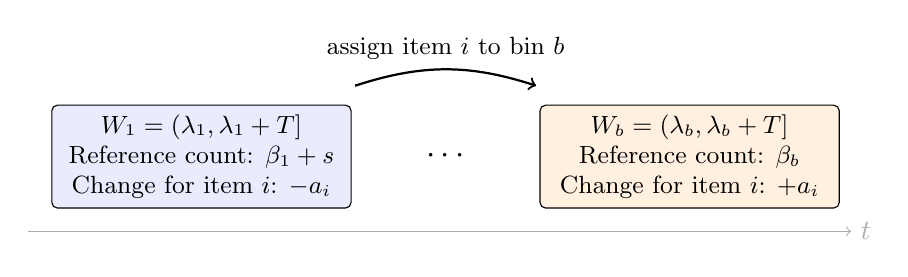
\begin{tikzpicture}[
  window/.style={draw,rounded corners=2pt,minimum width=3.8cm,
                 minimum height=1.15cm,align=center,font=\small}
]
  \node[window,fill=blue!8] (windowone) at (0,0)
    {$W_1=(\lambda_1,\lambda_1+T]$\\
     Reference count: $\beta_1+s$\\
     Change for item $i$: $-a_i$};
  \node[font=\large] at (3.1,0) {$\cdots$};
  \node[window,fill=orange!12] (windowb) at (6.2,0)
    {$W_b=(\lambda_b,\lambda_b+T]$\\
     Reference count: $\beta_b$\\
     Change for item $i$: $+a_i$};
  \draw[->,thick] (1.95,0.9) to[bend left=18]
    node[above,font=\small] {assign item $i$ to bin $b$}
    (4.25,0.9);
  \draw[->,gray!65] (-2.2,-0.95)--(8.25,-0.95)
    node[right] {$t$};
\end{tikzpicture}
\caption{Relative to the reference matching, assigning one item of
size $a_i$ from bin 1 to bin $b$ removes $a_i$ from the first
histogram window and adds $a_i$ to window $b$; intermediate windows
are unchanged. Superposing the item transfers gives
$N(t)=\beta_j+L_j$ throughout window
$W_j=(\lambda_j,\lambda_j+T]$.}
\label{fig:hardness-window-transfer}
\end{figure}

\subsection{Expected depth: an exact matching formula}

The expected-depth reduction needs no clouds. Each nonzero
hypothesis is one path vertex or one isolated vertex, and every
query isolates either a singleton or an adjacent pair.
The combinatorial choice is still a matching, but its objective
depends on how the resulting pairs are ordered.

For a finite positive weight vector $z$, keeping repeated values
as distinct entries, define the \emph{weighted completion sum} by
\[
 \mathcal C(z)=\sum_{j=1}^{|z|}jz_{(j)},
 \qquad z_{(1)}\ge\cdots\ge z_{(|z|)}.
\]
It equals the sum of the individual weights plus the smaller
weight for each unordered pair of entries: in decreasing order,
an earlier entry delays a later entry by one. Thus concatenating
vectors $u,v$ adds the cross contribution
$\sum_{i,j}\min\{u_i,v_j\}$.
Equivalently,
if $h_z(t)=|\{j:z_j\ge t\}|$, then
\begin{equation}\label{eq:completion-histogram}
 \mathcal C(z)=\int_0^\infty
                 \frac{h_z(t)(h_z(t)+1)}2\,dt.
\end{equation}
At height $t$, the first $h_z(t)$ ranks contribute
$1+\cdots+h_z(t)$; integrating those contributions proves the identity.

\begin{lemma}[Exact singleton/pair formula]\label{lem:pair-invoice}
Consider a \emph{linear forest}, meaning a disjoint union of paths
(isolated vertices are allowed), with vertices $1,\ldots,N$ ordered
component by component. Represent them and a distinguished hypothesis by
$(i,i^2)$, $0\le i\le N$. Supply $I_{i,i}$ for each nonzero vertex
and $I_{i,i+1}$ for each forest edge.
Give the distinguished hypothesis weight $\omega_0>0$ and the
others positive weights $\omega_v$.
For a matching $\mathcal M$, let $J(\mathcal M)$ be the vector
containing mass
$\omega_u+\omega_v$ for each matched pair and $\omega_v$ for each
unmatched vertex, retaining multiplicities when masses coincide.
The optimal unnormalized expected depth is
\begin{equation}\label{eq:pair-invoice}
 \min_{\mathcal M}
 \left\{\omega_0(N-|\mathcal M|)
       +\mathcal C(J(\mathcal M))
       +\sum_{\{u,v\}\in\mathcal M}(\omega_u+\omega_v)\right\}.
\end{equation}
If $\omega_0>N\sum_{v>0}\omega_v$, an optimal matching in this
formula has maximum cardinality.
\end{lemma}
\begin{proof}
Follow hypothesis $0$, which misses every supplied membership query.
The hypotheses first covered together are disjoint singletons
or adjacent pairs. The pairs form a matching $\mathcal M$,
and the spine has $N-|\mathcal M|$ queries.
A pair's hit branch requires exactly one additional query;
a singleton branch requires none.
This gives the first and third terms of \eqref{eq:pair-invoice}.

For the first-cover term, suppose masses $a<b$ occupy consecutive
positions $j,j+1$. Their contribution is
$ja+(j+1)b$ in that order and $jb+(j+1)a$ after swapping, a decrease
of $b-a$. Repeated exchanges show that nonincreasing mass is optimal.
Every such ordering is executable: query the selected pairs
and the singleton tests for the unmatched vertices in that order.
The groups are disjoint, so each query's hit branch exits only
to its own group. This proves the
formula both as a lower bound on arbitrary trees and as an
attainable value for each matching.

Every proper complete tree has depth at most $N$, so the total
weighted depth of all nonzero hypotheses is at most
$N\sum_{v>0}\omega_v$. One additional query on hypothesis $0$'s
path outweighs this entire budget under the stated inequality.
An optimal tree must consequently minimize that path's length,
which means choosing a maximum-cardinality matching.
\end{proof}

\subsection{Expected depth: bin loads become a quadratic penalty}

The formula above separates three effects: the distinguished
point's depth, first-cover positions, and one extra query for
each pair. We will force a maximum matching by making the
distinguished point sufficiently likely. Pair weights then
record the bin loads in disjoint histogram windows.
Small adjustments to the unmatched boundary weights cancel the
histogram's unwanted linear terms, leaving a quadratic penalty.

\begin{theorem}[Strong NP-completeness of expected depth]
\label{thm:strong-average}
Given supplied binary lines, a prior obtained by normalizing
strictly positive integer weights bounded by a fixed polynomial in
$n$, and a rational threshold $K$, deciding whether
$\OPT_{\mathrm E}(\HH)\le K$ is strongly NP-complete.
This holds for $\HH=\{(i,i^2):0\le i<n\}$, $O(n)$ supplied lines
with polynomially bounded integer coefficients, and even when each
query's negative class contains at most two hypotheses.
\end{theorem}
\begin{proof}
We again reduce from the restricted 3-Partition input.
In this proof put
\[
 q=2s(p-1),\qquad
 \beta_1=q-s,\qquad
 \beta_b=2s(p-b)\quad(2\le b\le p),\qquad
 a_{\max}=\max_i a_i.
\]
The integer $q$ is again the total matching size.
The $\beta_b$ will be the baseline pair counts in the bin windows.
Choose the explicit polynomial integers
\[
 \begin{split}
 r&=1000\bigl[(p+10)(q+m+1)^2
             +(qmp+2m+1)\beta_1a_{\max}+1\bigr],\\
 V&=2000m(r+q+m+1),\qquad Z=V/2,\qquad t_i=q+r+m-i,\\
 \delta_{ib}&=\left\lfloor
          \frac{V(\beta_1-\beta_b)a_i}{t_i}\right\rfloor,\qquad
 D=\max_{i,b}\delta_{ib},\qquad A_i=1+(2D+1)i,\\
 \lambda_b&=(10+2b)V\quad(1\le b\le p).
 \end{split}
\]
\begin{symboltable}
$q,\ \beta_b$ & Total matching size and baseline pair count in bin window $b$.\\
$r,\ V,\ Z=V/2$ & Number of medium-weight isolated hypotheses, window width, and isolated-hypothesis weight.\\
$t_i$ & Coefficient with which item $i$'s unmatched boundary weight contributes to the expected-depth objective.\\
$\delta_{ib},\ D$ & Boundary adjustment for item $i$ in bin $b$, and the largest such adjustment.\\
$A_i$ & Increasing base weight for item $i$'s unmatched boundary hypothesis.\\
$\lambda_b$ & Lower level of bin window $b$, separated from neighboring windows by $2V$.\\
$b_i,\ L_b$ & Bin assigned to item $i$ and total item size assigned to bin $b$.\\
$U_i,\ z,\ G$ & Unmatched item weights, matched-pair masses, and the resulting unnormalized weighted depth.\\
$G_{\mathrm{fix}},\ C_{\mathrm{ref}},\ e$ & Matching-independent cost, reference completion sum, and bounded rounding/perturbation error.\\
$E_+,\ E_-,\ k_0,\ k$ & Upper and lower error bounds, baseline threshold, and final decision threshold.\\
\end{symboltable}
For $b\ge2$,
$\beta_1-\beta_b=(2b-3)s>0$, so all $\delta_{ib}$ are
nonnegative; the formula gives $\delta_{i1}=0$.
The even-position vertices $E_{i,2a_i(b-1)}$ are the $p$ boundary
choices for item $i$; leaving boundary $b$ unmatched assigns that
item to bin $b$. Between consecutive boundaries are $2a_i$ steps,
with $a_i$ increases and $a_i$ decreases in the even weights.
The odd weights are chosen so the two possible pairings at an
increasing step have masses $\lambda_b$ and $\lambda_b+V$, while
those at a decreasing step have masses $\lambda_{b+1}+V$ and
$\lambda_{b+1}$. Moving the unmatched position across a segment
therefore transfers exactly $a_i$ pair masses from bin window $b$
to window $b+1$.

This transfer is the encoding invariant. The large window width $V$
makes a unit of load imbalance dominate all rounding errors. The
small boundary adjustments $\delta_{ib}$ will cancel the remaining
linear dependence on the chosen bins, leaving a quadratic penalty
that is zero exactly for a 3-partition.
The constants $1000$ and $2000$ provide slack in the scale
estimates below. The combinatorial information is carried by
the item lengths and the bin windows, not by those constants.

\paragraph{Step 1: construct the weighted item paths.}
For item $i$, form an odd path
\[
 E_{i0},\,B_{i1},\,E_{i1},\,\ldots,\,
 B_{is_i},\,E_{is_i},\qquad s_i=2a_i(p-1),
\]
where each displayed symbol also denotes that vertex's weight.
First define unperturbed even weights
\[
 E^0_{ij}=
 \begin{cases}
 A_i,&j\equiv0\pmod{2a_i},\\
 A_i+V,&j\text{ odd},\\
 A_i+2V,&\text{otherwise}.
 \end{cases}
\]
Each consecutive difference is $+V$ or $-V$.
Between two boundary positions there are $2a_i$ steps,
of which $a_i$ go up and $a_i$ go down.
For $1\le j\le s_i$ let $b=\lceil j/(2a_i)\rceil$ and put
\[
 B_{ij}=
 \begin{cases}
 \lambda_b-E^0_{i,j-1},&E^0_{ij}-E^0_{i,j-1}=V,\\
 \lambda_{b+1}-E^0_{ij},&E^0_{ij}-E^0_{i,j-1}=-V.
 \end{cases}
\]
Finally set
$E_{i,2a_i(b-1)}=A_i+\delta_{ib}$ at each of the $p$ boundaries
and leave all other even weights unperturbed.
The odd weights do not change when this adjustment is made.

Add $r$ isolated forest vertices of weight $Z$.
The nonzero forest has $N=2q+m+r$ vertices, with maximum matching
size $q$. Let $P$ be the total weight of its item-path vertices,
$W=P+rZ$, and give hypothesis $0$ weight
$\omega_0=(N+1)W+1$.
Use precisely the lines of Lemma~\ref{lem:pair-invoice}.
Normalize the weights only after the construction.

\paragraph{Step 2: verify the separation between weight scales.}
\begin{claim}[The chosen parameters separate the weight scales]
\begin{equation}\label{eq:expected-scale-bounds}
 \begin{split}
 \max_{i,b}(A_i+\delta_{ib})&<V/100,\\
 E_+ :=q\sum_{i,b}\delta_{ib}&\le V/1000,\\
 E_- :=\sum_i(t_i-1)&<V/2000.
 \end{split}
\end{equation}
\end{claim}
\begin{proof}
Indeed, $t_i\ge r$ gives $D\le V\beta_1a_{\max}/r$.
Consequently,
\[
 E_+\le qmpD\le V/1000,
 \qquad
 \max_{i,b}(A_i+\delta_{ib})
 \le(2m+1)D+m+1
 \le V/1000+V/2000<V/100.
\]
The bound $m+1\le V/2000$ follows directly from
$V=2000m(r+q+m+1)$.
Also $t_i-1<r+q+m+1$, giving
$E_-<m(r+q+m+1)=V/2000$.
\end{proof}
The first bound keeps every boundary singleton below $Z$ and fixes
the order of the unmatched item weights. The second limits the total
change in pair-mass completion cost caused by the perturbations; the
third bounds the accumulated error from the floors. The large $r$
is chosen to make all three estimates hold with room to spare.

Every even weight is positive. By the first bound in
\eqref{eq:expected-scale-bounds}, $A_i+\delta_{ib}<V/100$, so
$A_i+2V<2.01V$ and every unmatched even weight is below $3V$.
For an upward step, the two possible pair masses are
$\lambda_b$ and $\lambda_b+V$; for a downward step they are
$\lambda_{b+1}+V$ and $\lambda_{b+1}$. Since
$\lambda_b\ge12V$ and $\lambda_{b+1}\ge14V$, all these masses are
at least $12V$. Boundary adjustments are nonnegative and can only
increase a matched pair's mass. The odd weights are also positive:
each is either $\lambda_b-E^0_{i,j-1}$ or
$\lambda_{b+1}-E^0_{ij}$, and every unperturbed even weight is
less than $2.01V$. Hence every pair mass exceeds $Z=V/2$ and every
unmatched even weight.
Lemma~\ref{lem:pair-invoice} restricts the optimum to maximum
matchings. By Lemma~\ref{lem:odd-path}, each item then leaves
one even vertex unmatched.

\paragraph{Step 3: isolate the matching-dependent terms.}
Write $U=(U_1,\ldots,U_m)$ for the unmatched weights and $z$ for
the $q$ pair masses. Their exact weighted depth is
\begin{claim}[Expected-depth invoice for a fixed matching]
\begin{equation}\label{eq:expected-remaining-invoice}
 G=G_{\mathrm{fix}}+\mathcal C(z)+\mathcal C(U)
       +(q-1)\sum_i U_i+r\sum_i\min\{U_i,Z\},
\end{equation}
where
\[
 G_{\mathrm{fix}}=
 \omega_0(q+m+r)+\frac{Zr(r+1)}2+qrZ+P.
\]
\end{claim}
\begin{proof}
To derive this expression, split the completion sum into the
three groups $z,U$, and the $r$ isolated weights $Z$.
Since every pair mass is larger than the other weights, their
cross terms are $qrZ$ and $q\sum_iU_i$.
The remaining cross term is $r\sum_i\min\{U_i,Z\}$.
Identifying the pairs adds their total weight
$P-\sum_iU_i$, which changes the coefficient $q$ to $q-1$.
The distinguished path contributes $\omega_0(q+m+r)$.
Everything not depending on the matching is collected in
$G_{\mathrm{fix}}$.
\end{proof}

\paragraph{Step 4: compute what a boundary choice changes.}
\begin{claim}[Pair-mass windows encode the bin loads]
Let $b_i$ be the bin chosen by item $i$ and
$L_b=\sum_{i:b_i=b}a_i$. Let $z^0$ be the unperturbed pair-mass
vector for these choices, and let $C_{\mathrm{ref}}$ be the
completion sum of the reference vector in which every item chooses
bin $1$. Then
\begin{equation}\label{eq:expected-bin-identity}
 \mathcal C(z^0)=C_{\mathrm{ref}}+
 V\left[\sum_b\beta_bL_b-\beta_1s+
             \frac{\sum_bL_b^2-s^2}{2}\right].
\end{equation}
\end{claim}
\begin{proof}
Unmatching boundary $2a_i(b-1)$ assigns item $i$ to bin $b$.
Temporarily omit the boundary perturbations and denote the
resulting pair-mass vector by $z^0$.
For an upward step in segment $b$, pairing its odd vertex
to the even vertex on the left gives mass $\lambda_b$,
while pairing right gives $\lambda_b+V$.
For a downward step, those masses are
$\lambda_{b+1}+V$ and $\lambda_{b+1}$.
Moving the unmatched vertex across a whole segment consequently
changes the pair-mass histogram by
\[
 -a_i\mathbf1_{(\lambda_b,\lambda_b+V]}+
  a_i\mathbf1_{(\lambda_{b+1},\lambda_{b+1}+V]}.
\]
There are exactly $a_i$ steps of each type.
As in the maximum-depth construction, transfers across consecutive
segments cancel except at the starting and chosen bins.
In the reference matching, all odd vertices are paired to their
right. Segment $b$ contributes $s$ masses $\lambda_b+V$ and
$s$ masses $\lambda_{b+1}$ after summing over items.
For thresholds $t$ in the first window, the reference tail count
is $q=\beta_1+s$; for later window $b$ it is
$2s(p-b)=\beta_b$. Assigning items according to loads $L_b$
changes the tail count throughout window $b$ to
$\beta_b+L_b$: the first window loses $s-L_1$ pair masses from its
reference count $q$, while each later window gains $L_b$.
Outside these disjoint windows the tail histogram is unchanged.

Let $C_{\mathrm{ref}}$ be the completion sum of the unperturbed
pair masses when every first boundary is unmatched. It is explicitly
computable by sorting those $q$ masses.
Within a window the integrand of
\eqref{eq:completion-histogram} is the triangular polynomial
$h(h+1)/2$. Substituting $h=\beta_b+L_b$ and subtracting the
reference loads $(s,0,\ldots,0)$ gives the following expression.
For a baseline count $\beta_b$, the change in the triangular
polynomial is
$\beta_bL_b+(L_b^2+L_b)/2$. The reference has load $s$ in the first
window, so its change is
$\beta_1s+(s^2+s)/2$. Subtracting this reference change cancels the
linear $L_b/2$ terms because $\sum_bL_b=s$.
The remaining expression has a useful quadratic term, but also
the unwanted linear term $\sum_b\beta_bL_b$.
\end{proof}

\paragraph{Step 5: cancel the linear term and bound rounding.}
\begin{claim}[Boundary adjustments leave only a bounded error]
For every boundary matching, there is an error $e$ with
$-E_-\le e\le E_+$ such that
\begin{equation}\label{eq:expected-quadratic-gap}
 G=G_{\mathrm{fix}}+\sum_i t_iA_i+C_{\mathrm{ref}}+
       \frac V2\left(\sum_bL_b^2-s^2\right)+e.
\end{equation}
\end{claim}
\begin{proof}
Boundary perturbations increase pair masses by at most the total
added boundary weight. For a vector $z$ of $q$ pair masses,
$\mathcal C(z)=\min_\sigma\sum_{j=1}^q jz_{\sigma(j)}$, by the
adjacent-swap ordering argument in Lemma~\ref{lem:pair-invoice}.
If coordinates increase by a total
amount $\Delta$, this representation shows that $\mathcal C$ is
nondecreasing and increases by at most $q\Delta$: evaluate the new
vector in an ordering optimal for the old one. Here
$\Delta\le\sum_{i,b}\delta_{ib}$, so the increase is at most
$q\sum_{i,b}\delta_{ib}=E_+$.
All boundary unmatched weights are below $Z$, and their order is
the fixed decreasing item order. Indeed,
$A_{i+1}-(A_i+D)=D+1>0$, so even the largest perturbation of item
$i$ leaves it below the unperturbed weight of item $i+1$.
Thus their terms in \eqref{eq:expected-remaining-invoice} are
$\sum_i t_i(A_i+\delta_{ib_i})$.
Indeed, item $i$ has rank $m-i+1$ in $\mathcal C(U)$, plus
coefficient $q-1+r$ from the other terms, giving $t_i=q+r+m-i$.
The floor definition gives
\[
 -E_-\le
 \sum_i t_i\delta_{ib_i}
       -V\sum_i(\beta_1-\beta_{b_i})a_i
 \le0.
\]
For each item, the difference is minus the remainder when the
integer $V(\beta_1-\beta_{b_i})a_i$ is divided by $t_i$; its
magnitude is therefore at most $t_i-1$.
Its intended contribution
$V\sum_i(\beta_1-\beta_{b_i})a_i$ cancels the unwanted linear
term in \eqref{eq:expected-bin-identity}.
Each floor loses an integer between zero and $t_i-1$.
Combining that loss with the pair-mass increase gives
the claimed error interval.
\end{proof}

\paragraph{Step 6: distinguish exact balance by a quadratic gap.}
\begin{claim}[The quadratic gap detects a 3-partition]
For boundary choices, the threshold $k$ is met exactly when every
bin load is $B$.
\end{claim}
\begin{proof}
Define the integer threshold
\[
 k_0=G_{\mathrm{fix}}+\sum_i t_iA_i+C_{\mathrm{ref}}+
              \frac V2(pB^2-s^2),\qquad k=k_0+E_+.
\]
Because $\sum_bL_b=pB$,
\[
 \sum_bL_b^2-pB^2=\sum_b(L_b-B)^2.
\]
A source partition makes this sum zero and gives weighted depth
at most $k$. Otherwise the integral deviations sum to zero and
include at least one positive and one negative entry. Their
squares sum to at least two.
The weighted depth is then at least $k_0+V-E_-$.
The scale bounds give
$V-E_->1999V/2000>V/1000\ge E_+$, so this depth exceeds
$k=k_0+E_+$.
\end{proof}

\paragraph{Step 7: exclude internal unmatched vertices.}
\begin{claim}[An internal unmatched vertex exceeds the threshold]
Every maximum matching that leaves an internal even-position item
vertex unmatched has weighted depth greater than $k$.
\end{claim}
\begin{proof}
The preceding calculation concerned boundary choices. To complete
soundness, a maximum matching leaving an internal even vertex
unmatched must also exceed $k$.
Such a vertex has weight $A_i+V$ or $A_i+2V$, exceeding $Z$.
Every other unmatched weight is at least its $A_i$.
Its interactions with the $r$ isolated vertices contribute $rZ$
instead of at least $rA_i$. The other matching-dependent terms
in \eqref{eq:expected-remaining-invoice} are nonnegative, so
\[
 G\ge G_{\mathrm{fix}}+r\sum_i A_i+
                   r\bigl(Z-\max_i A_i\bigr).
\]
On the other hand, $pB^2-s^2\le0$ gives
\[
 k\le G_{\mathrm{fix}}+r\sum_i A_i+
           C_{\mathrm{ref}}+(q+m)\sum_i A_i+E_+.
\]
The reference masses are at most $(11+2p)V$, so
$C_{\mathrm{ref}}\le(p+6)(q+1)^2V$.
Using $A_i<V/100$, the last three terms are less than
$(p+8)(q+m+1)^2V$.
But $Z-\max_i A_i>V/3$ and
$r\ge1000(p+10)(q+m+1)^2$.
The lower bound for an internal unmatched vertex is therefore
strictly larger than $k$.
\end{proof}
Thus the medium-weight isolated hypotheses exclude all internal
choices. Soundness now covers every maximum matching, and
Lemma~\ref{lem:pair-invoice} makes this sufficient for arbitrary
adaptive trees.

\paragraph{Size, positive priors, and membership in NP.}
Normalize the positive weights by their total $\Omega$ and use
the expected-depth threshold $k/\Omega$.
The construction has polynomial size on the restricted source input.
With $n=N+1$, we have $V=O(n^2)$, all nonzero vertex weights are
$O(n^3)$, and $\omega_0=O(n^5)$.
Coordinates and supplied-line coefficients are $O(n^2)$ and there
are $O(n)$ queries. Membership in NP follows by evaluating a
proper complete tree with $n-1$ internal nodes.
Both the normalized priors and the threshold have polynomially
bounded integer numerators and denominators. This establishes
strong NP-completeness with strictly positive polynomially bounded
hypothesis weights.
\end{proof}

